
\documentclass[fleqn,addpoints]{exam}
\usepackage{amsmath}
\usepackage{graphicx}
\usepackage{booktabs}
\usepackage{float}
\usepackage{caption}
\usepackage{polynom}
\usepackage{mdwlist}
\usepackage{cancel}

\usepackage{unitsdef} 
\newunit{\inch}{in}
\newunit{\mile}{mile}
\newunit{\mph}{mph}
\newunit{\foot}{ft}
\newunit{\knot}{knot}
\newunit{\gallon}{gallon}

\bracketedpoints
\everymath{\displaystyle}

\printanswers

% \begin{figure}[H]
%   \centering
%   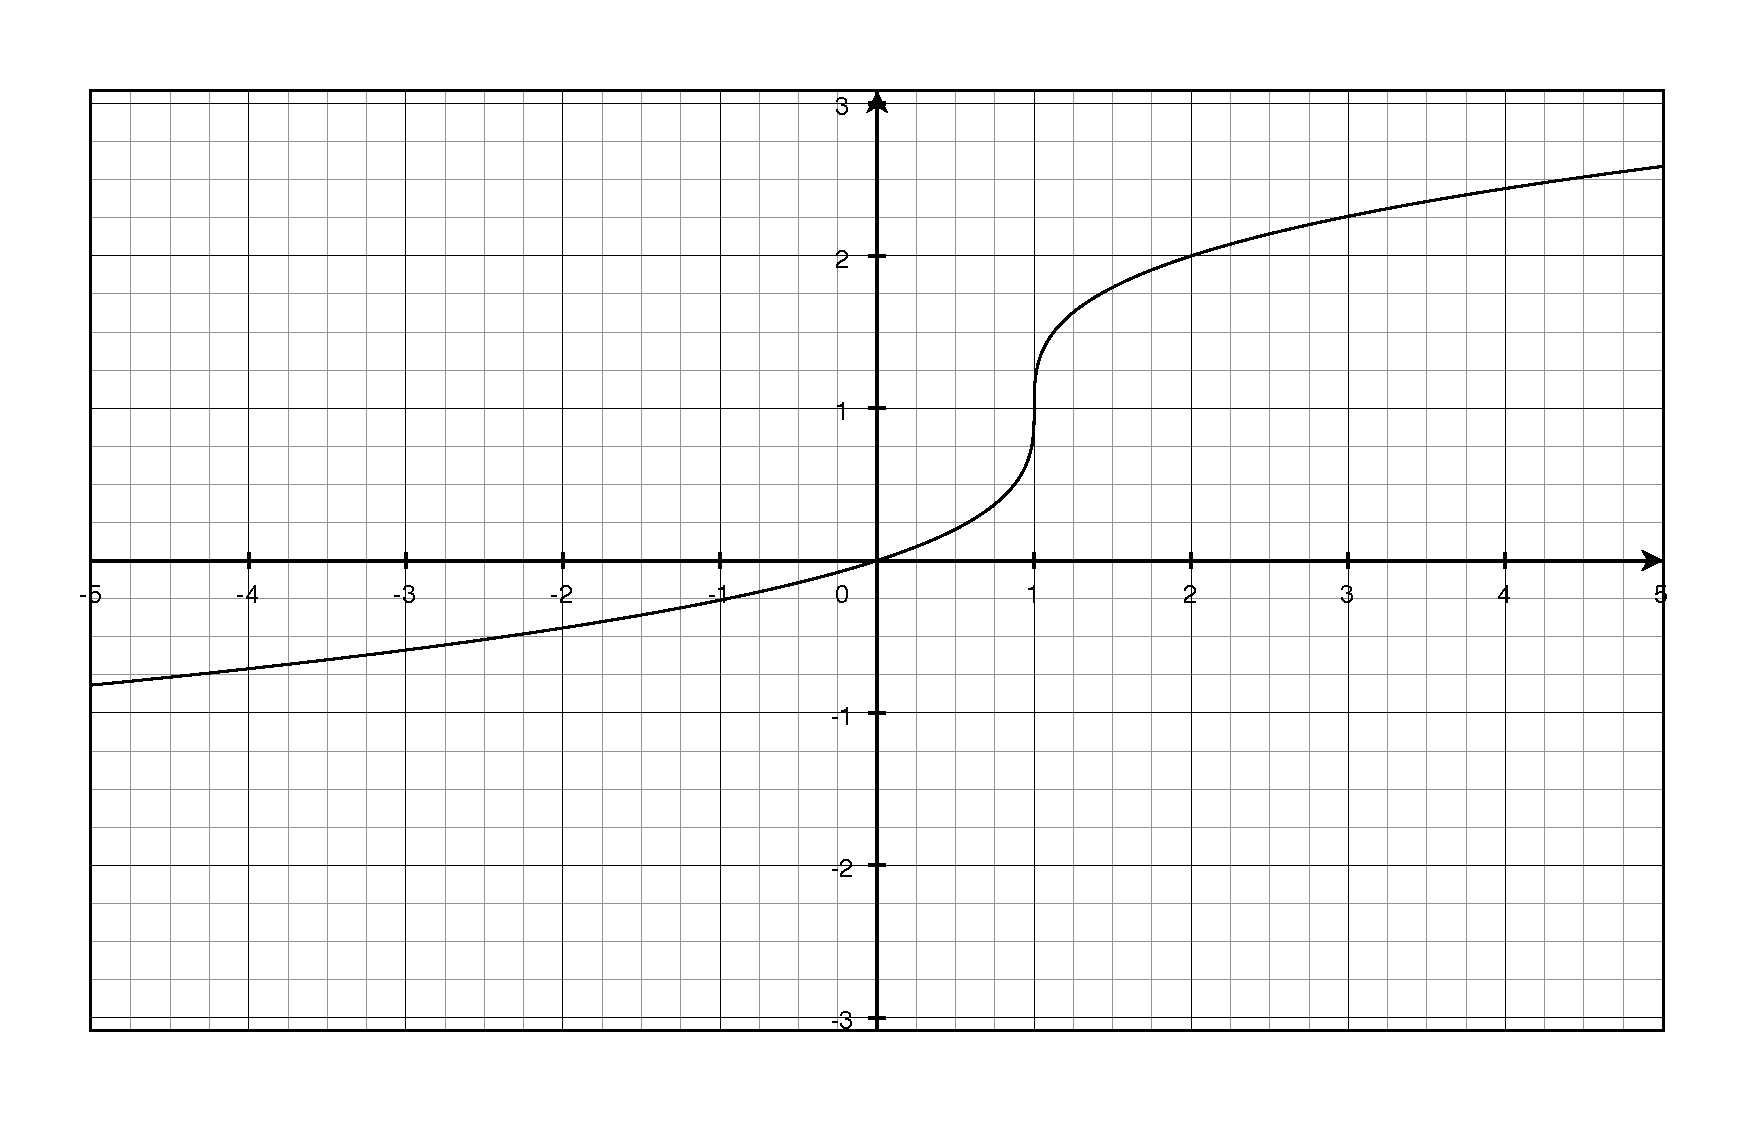
\includegraphics[scale=.3]{question7.eps}
%   \caption*{Question 7}
% \end{figure}

% \begin{tabular}{cc}
% \toprule
% period & amplitude \\
% \midrule
%   $\pi$ & $2$ \\
% \bottomrule
% \end{tabular}

\ifprintanswers
\usepackage{2in1, lscape}
\fi

% from Winter and Spring 2011 final

\title{Math 263A Sample Final Seven}

\date{November 15, 2012}

\author{}

\begin{document}

\maketitle  

{\em This final is a mix of questions from two OU finals.}

\begin{questions}

\question Sketch the graph of a function that:
\begin{itemize*}
\item has a removable (point) discontinuity at $x = 0$
\item has a jump discontinuity at $x = 1$
\item has a vertical asymptote at $x = -1$ 
\item has a horizontal asymptote at $y = 2$
\item is continuous elsewhere
\end{itemize*}

\begin{solution}
  My computer can't draw these.
\end{solution}

\question Sketch the graph of a function $f$ that satisfies all of the given conditions: 
\begin{itemize*}
\item $f(1) = 2$
\item $f'(x)$ is always positive
\item $f''(x)$ is always negative
\item $f(x)$ has a horizontal asymptote at $y = 5$ as $x \rightarrow +\infty$
\end{itemize*}

\begin{solution}
  My computer can't draw these.
\end{solution}

\ifprintanswers
\pagebreak
\fi

\question Find the limit, if it exists. If the limit does not exist, explain why.
\[
  \lim_{x \to 3} \frac{x^2 - 2x - 3}{x - 3}
\]

\begin{solution}
\begin{align*}
  \lim_{x \to 3} \frac{x^2 - 2x - 3}{x - 3} &= \lim_{x \to 3} \frac{\cancel{(x - 3)}(x + 1)}{\cancel{x - 3}} \\
    &= \lim_{x \to 3} (x + 1) \\
    &= 4 \\
\end{align*}

\end{solution}

\question The area of a circle is increasing at a rate of $5 \meter^2/\second$. What is the rate of change of the radius of the
circle (in m/s) when the area is $10^4 \pi \meter^2$?

\begin{solution}
\begin{align*}
  A &= \pi r^2 \\
  \frac{dA}{dt} &= 2 \pi r \frac{dr}{dt} \\
  \frac{dr}{dt} &= \frac{1}{2 \pi r} \frac{dA}{dt} \\
\end{align*}

We need to find the radius for the time when the area is $10^4 \pi \meter^2$:
\begin{align*}
  A &= \pi r^2 \\
  r &= \sqrt{\frac{A}{\pi}} \\
    &= \sqrt{\frac{10^4 \pi}{\pi}} \\
    &= 100 \meter \\
\end{align*}

Now we can find the rate:
\begin{align*}
  \frac{dr}{dt} &= \frac{1}{2 \pi \cdot 100} \cdot 5 \\
  &= \frac{1}{40 \pi} \meter / \second \\
\end{align*}

\end{solution}
\question Find the linearization (linear approximation) of the function $f(x) = \sqrt{1 + x}$ at $x = 0$ and use
it to approximate the numbers $\sqrt{1.1}$ and $\sqrt{1.01}$.

\begin{solution}
\begin{align*}
  y &= (x + 1)^{1/2} \\
  \frac{dy}{dx} &= \frac{1}{2} (x + 1)^{-1/2} \\
  dy &= \frac{dx}{2 \sqrt{x + 1}}
\end{align*}

\begin{tabular}{cc}
\toprule
dx & dy \\
\midrule
$0.1$  & $0.05$ \\
$0.01$ & $0.005$ \\
\bottomrule
\end{tabular}

\begin{align*}
  \sqrt{1.1} \approx 1.05 \\
  \sqrt{1.01} \approx 1.005 \\
\end{align*}

\end{solution}

\ifprintanswers
\pagebreak
\fi

\question Find the derivative of the function {\em using the definition of derivative}. Check your answer using
differentiation rules. State the domain of the function and the domain of the derivative.
\[
  f(x) = \sqrt{x}
\]

\begin{solution}
\begin{align*}
  f'(x) &= \lim_{h \to 0} \frac{\sqrt{x + h} - \sqrt{x}}{h} \\
        &= \lim_{h \to 0} \frac{\sqrt{x + h} - \sqrt{x}}{h} \cdot \frac{\sqrt{x + h} + \sqrt{x}}{\sqrt{x + h} + \sqrt{x}} \\
        &= \lim_{h \to 0} \frac{x + h - x}{h (\sqrt{x + h} + \sqrt{x})} \\
        &= \lim_{h \to 0} \frac{\cancel{h}}{\cancel{h} (\sqrt{x + h} + \sqrt{x})} \\
        &= \lim_{h \to 0} \frac{1}{\sqrt{x + h} + \sqrt{x}} \\
        &= \frac{1}{2 \sqrt{x}} \\
\end{align*}

using differentiation rules:
\begin{align*}
  f(x) &= x^{1/2} \\
  f'(x) &= \frac{1}{2} x^{-1/2} \\
        &= \frac{1}{2 \sqrt{x}} \\
\end{align*}

The domain of the function is $[0, \infty)$ and the domain of the derivative is $(0, \infty)$.

\end{solution}

\ifprintanswers
\pagebreak
\fi

\question Use implicit differentiation to find an equation of the tangent line to the curve at $(1, 1)$.
\[
  x^2 + xy + y^2 = 3
\]
\begin{solution}
find the derivative
\begin{align*}
  x^2 + xy + y^2 &= 3 \\
  2x + xy' + y + 2yy' &= 0 \\
  y'(x + 2y) &= -2x - y \\
  y' &= \frac{-2x - y}{x + 2y} \\
\end{align*}

find the slope at $(1, 1)$:
\[
  m = \frac{-2 -1}{1 + 2} = -1
\]

find the equation for the line:
\begin{align*}
  y - 1 &= -1(x - 1) \\
  y - 1 &= -x + 1 \\
  y &= -x + 2 \\
\end{align*}

The question didn't ask for the graph, but here it is anyway:
\begin{figure}[H]
  \centering
  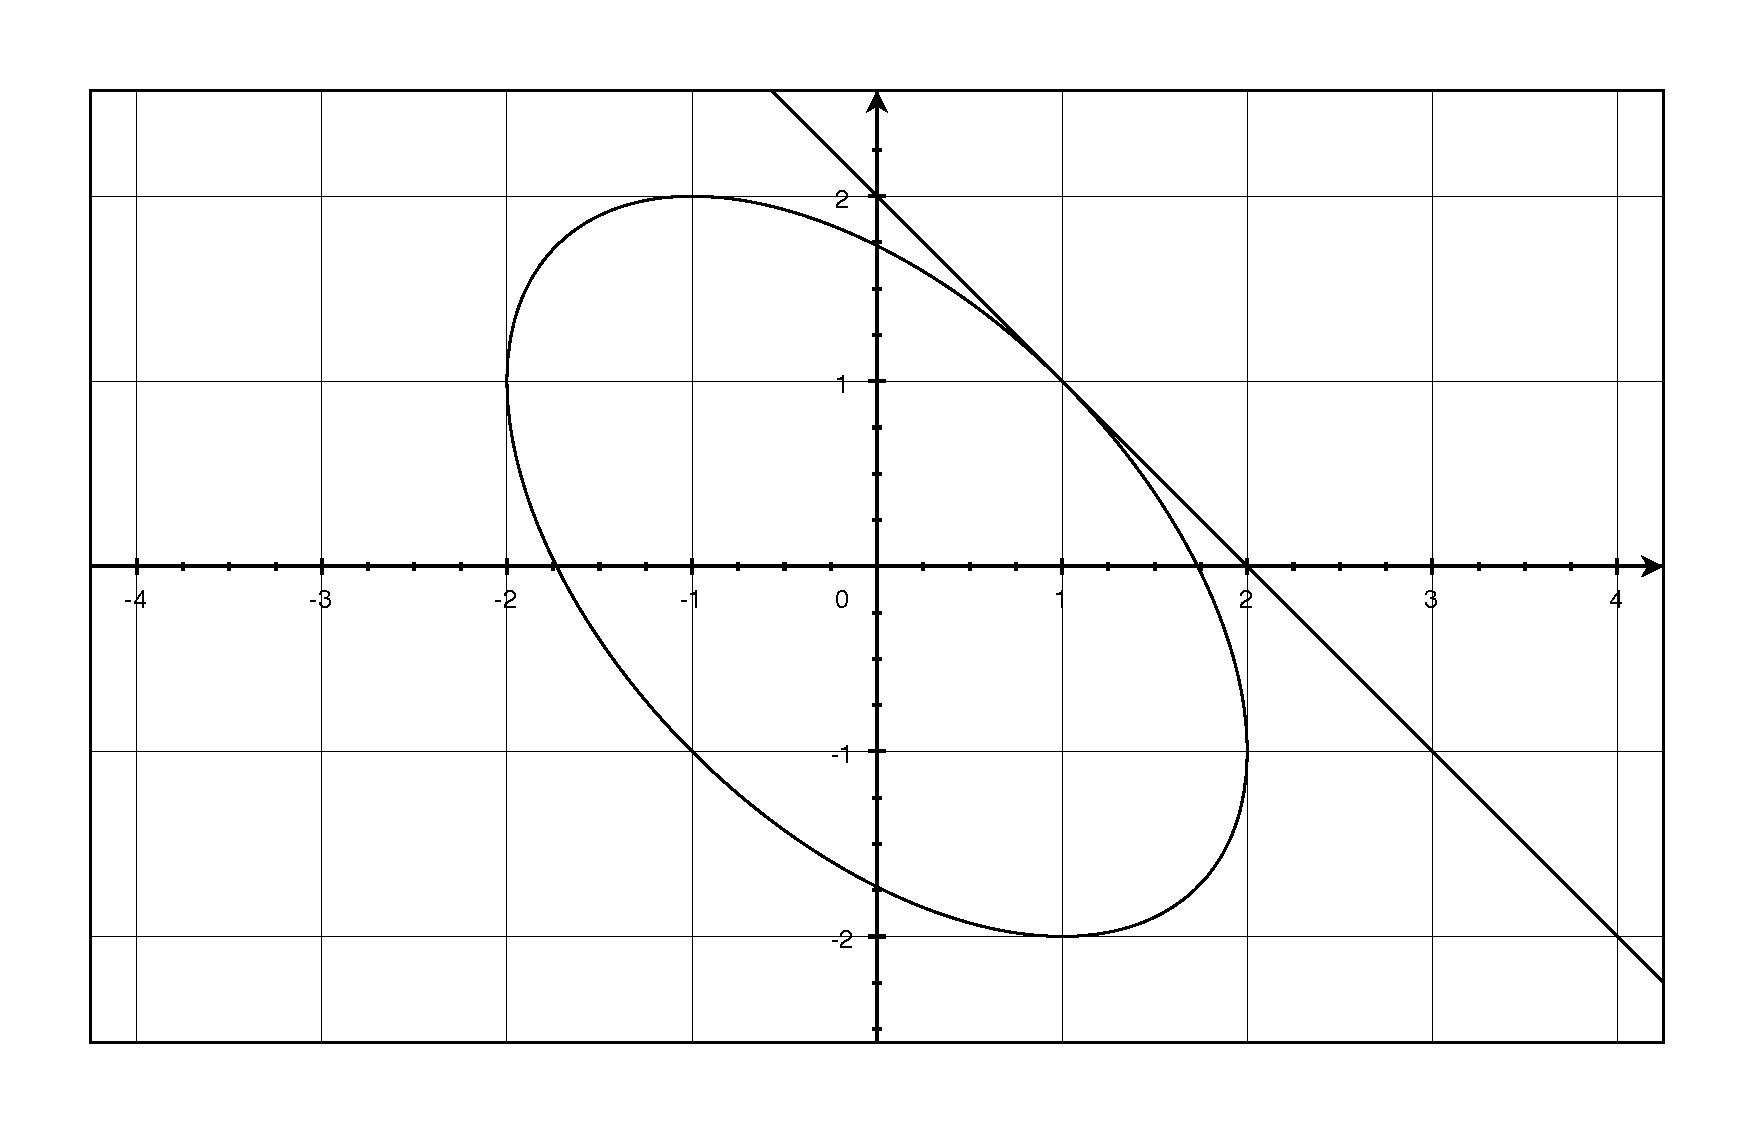
\includegraphics[scale=.3]{final_7_q7.eps}
  \caption*{Question 7}
\end{figure}
\end{solution}

\question Find the derivative of the function and an equation of the tangent line at $x = 1$:
\[
  y = \sin(x - 1)
\]

\begin{solution}
Find the derivative:
\[
  y' = \cos(x - 1)
\]

Find the slope at $x = 1$:
\[
  m = \cos(1 - 1) = \cos 0 = 1
\]

Find the y value for $x = 1$:
\begin{align*}
  y = \sin(1 - 1) = \sin 0 = 0
\end{align*}

Now we have the slope and a point, we can get an equation for the line:
\begin{align*}
  y - 0 &= 1(x - 1) \\
  y &= x - 1 \\
\end{align*}

Here's the graph (not asked for in the question):
\begin{figure}[H]
  \centering
  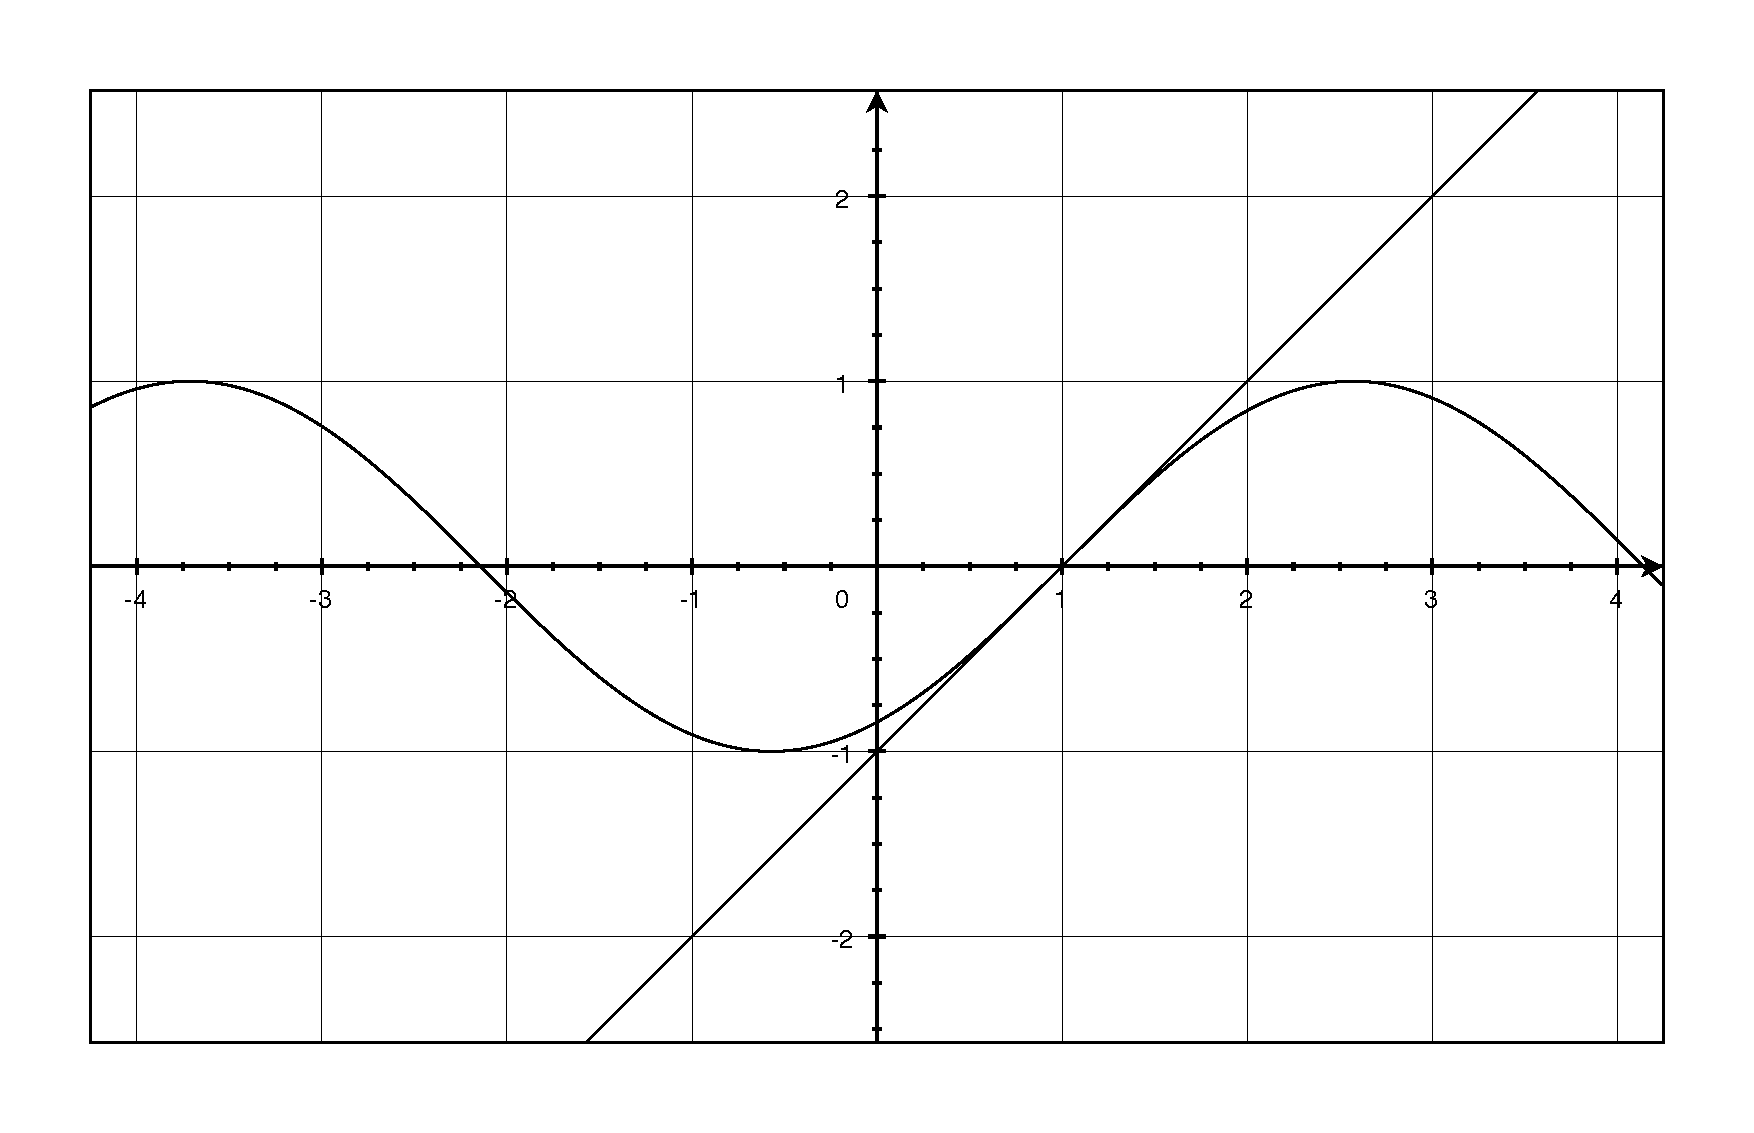
\includegraphics[scale=.3]{final_7_q8.eps}
  \caption*{Question 8}
\end{figure}

\end{solution}

\question Find the absolute maximum and minimum values of $f$ on the given interval.
\[
  f(x) = x^3 - 3x^2 + 1 \text{; } [-1, 3]
\]
\begin{solution}
Find the derivative:
\[
  f'(x) = 3x^2 - 6x
\]

Find the critical points:
\begin{align*}
  3x^2 - 6x &= 0 \\
  x^2 - 2x &= 0 \\
  x(x - 2) &= 0 \\
  x &= \{0, 2\} \\
\end{align*}

Try all the interesting points to find the minimum and maximum
\begin{tabular}{cc}
\toprule
$x$ & $f(x)$ \\
\midrule
$-1$  & $-3$ \\
$0$  & $1$ \\
$2$  & $-3$ \\
$3$  & $1$ \\
\bottomrule
\end{tabular}

So the minimums and maximums are:
\begin{itemize*}
\item minimums: $(-1, -3)$ and $(2, -3)$
\item maximums: $(0, 1)$ and $(3, 1)$
\end{itemize*}

\begin{figure}[H]
  \centering
  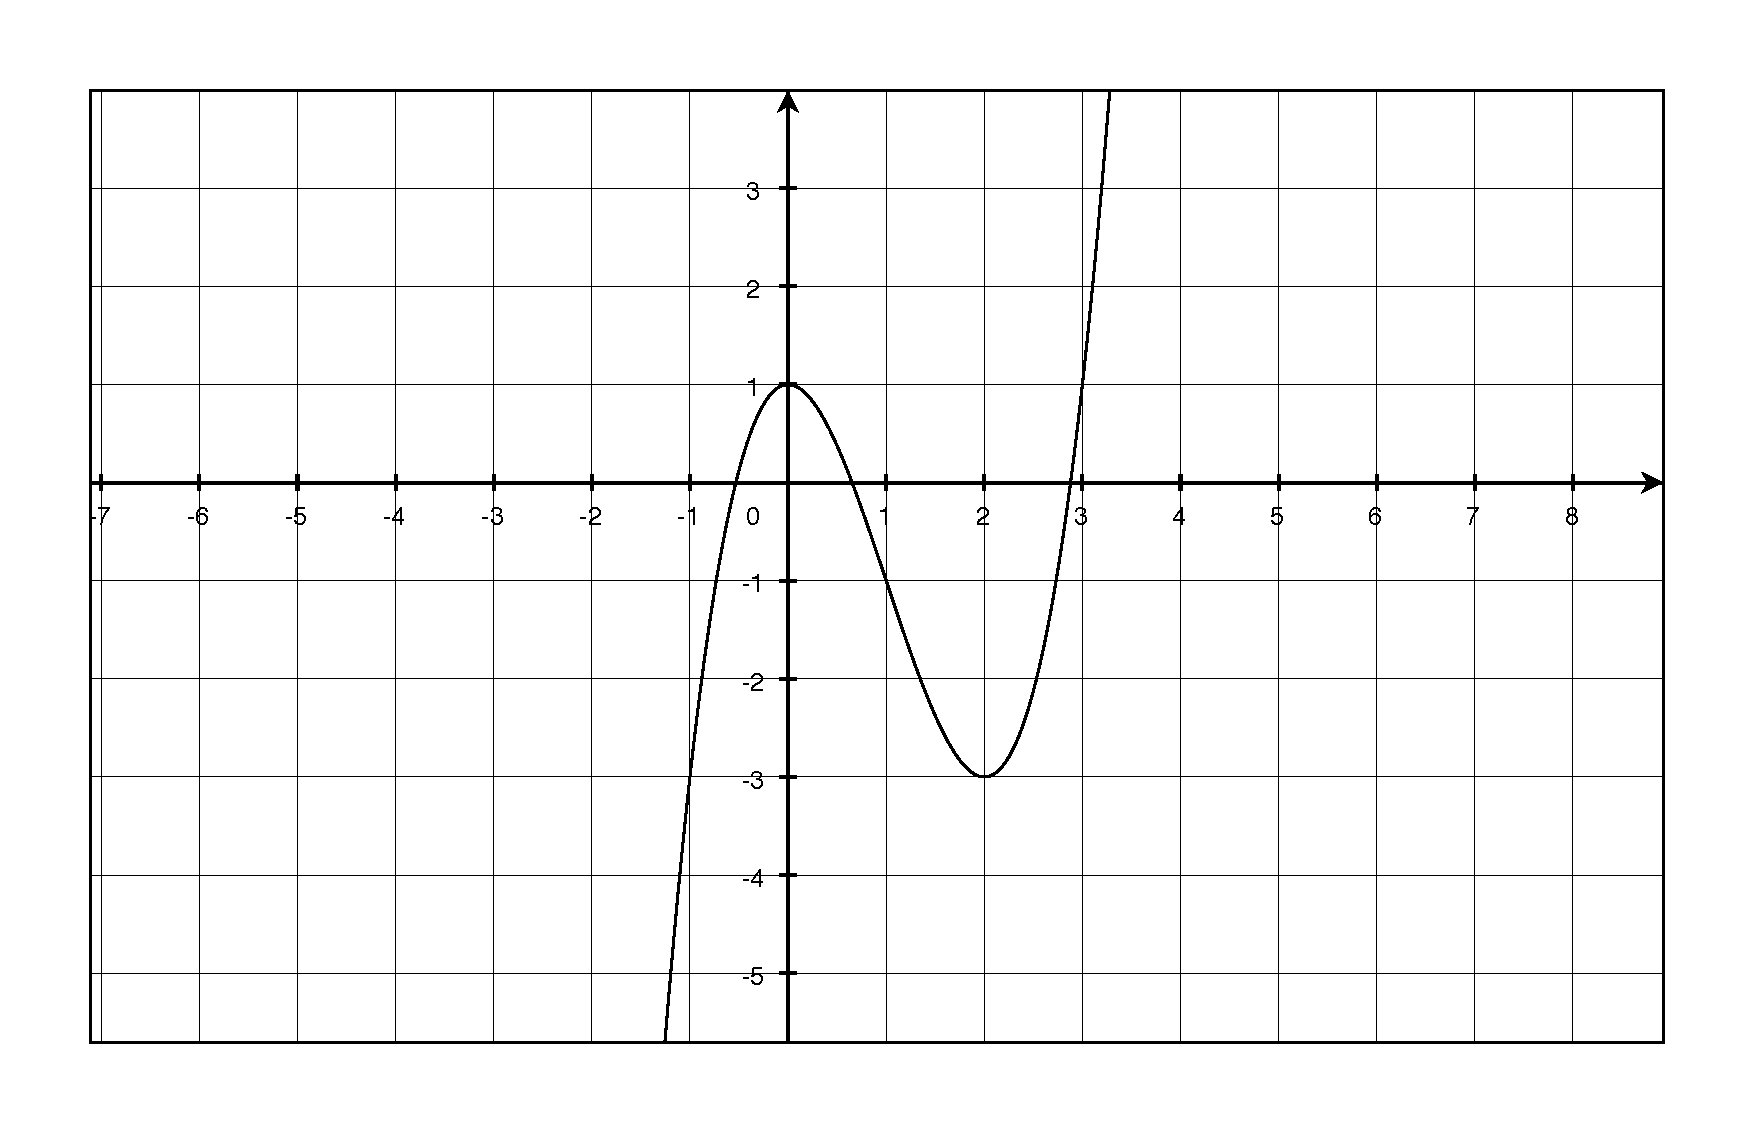
\includegraphics[scale=.3]{final_7_q9.eps}
  \caption*{Question 9}
\end{figure}
\end{solution}

\ifprintanswers
\pagebreak
\fi

\question Find the derivatives of the functions:
\begin{parts}
\part $f(x) = (2x)^{100} + 4 \pi^2$
\begin{solution}
{\em approach 1}
\begin{align*}
  f(x) &= (2x)^{100} + 4 \pi^2 \\
       &= 2^100 x^{100} + 4 \pi^2 \\
  f'(x) &= 100 \cdot 2^100 x^{99} \\
\end{align*}

{\em approach 2}
\begin{align*}
  f(x) &= (2x)^{100} + 4 \pi^2 \\
  f'(x) &= 100 \cdot (2x)^{99} \cdot 2 \\
        &= 100 \cdot 2^{99} x^{99} \cdot 2 \\
        &= 100 \cdot 2^{100} x^{99} \\
\end{align*}

\end{solution}

\part $g(u) = \frac{\tan u}{u}$
\begin{solution}
\begin{align*}
  g(u) &= \frac{\tan u}{u} \\
  g'(u) &= \frac{u \sec^2 u - \tan u}{u^2}
\end{align*}

\end{solution}

\end{parts}

\question Find the derivatives of the functions:
\begin{parts}
\part $f(t) = \frac{1}{(t^4 + 1)^3}$
\begin{solution}
\begin{align*}
  f(t) &= (t^4 + 1)^{-3} \\
  f'(t) &= -3(t^4 + 1)^{-4} \cdot 4t^3 \\
        &= \frac{-12 t^3}{(t^4 + 1)^4}
\end{align*}

\end{solution}

\part $g(x) = \cos^3 x$
\begin{solution}
\begin{align*}
  g(x) &= \cos^3 x \\
  g'(x) &= 3 \cos^2 x \cdot (- \sin x) \\
        &= - 3 \cos^2 x \sin x \\
\end{align*}
\end{solution}

\end{parts}

\question Differentiate:
\[
  \frac{x^2 + 4x + 3}{\sqrt{x}}
\]

\begin{solution}
{\em approach 1}
\begin{align*}
  f(x) &= \frac{x^2 + 4x + 3}{\sqrt{x}} \\
       &= x^{3/2} + 4x^{1/2} + 3x^{-1/2} \\
  f'(x) &= \frac{3}{2}x^{1/2} + 2x^{-1/2} - \frac{3}{2} x^{-3/2} \\
        &= \frac{3}{2}x^{1/2} + 2x^{-1/2} - \frac{3}{2} x^{-3/2} \\
\end{align*}

\end{solution}

\ifprintanswers
\pagebreak
\fi

\question Write the composite function in the form $f(g(x))$. Identify the inner function $u = g(x)$ and the outer function $y =
f(u)$. Then find the derivative $\frac{dy}{dx}$.  
\[
   y = (1 - x^2)^{10}
\]

\begin{solution}
I find writing the function in the way described in this problem not helpful and a bit confusing.  But anyway, here it
is:
\begin{align*}
  u(x) &= 1 - x^2 \\
  f(u) &= u^{10} \\
\end{align*}

With that out of the way, we can find the derivative of the original function:
\begin{align*}
  y' &= 10(1 - x^2)^9 \cdot D_x (1 - x^2) \\
     &= 10(1 - x^2)^9 \cdot (-2x) \\
     &= -20x (1 - x^2)^9 \\
\end{align*}


\end{solution}

\ifprintanswers
\pagebreak
\fi

\question Use the {\em Intermediate Value Theorem} to prove that there is a root of the given equation in
the interval $(0, 1)$.
\[
  \cos x = x
\]

\begin{solution}
The function is: $f(x) = \cos x - x$.  What we need to do is verify that the function is positive at one end of the
interval and negative at the other end:
\begin{align*}
  f(0) &= \cos 0 - 0 = 1 > 0 \\
  f(1) &= \cos 1 - 1 < 0 \\
\end{align*}

So the function must cross the x-axis somewhere between $x = 0$ and $x = 1$ and there is a root in this interval.
So by the  is a root

\end{solution}

\question
If $V$ is the volume of a cube with edge length $x$ and the cube expands as time passes, find
$\frac{dV}{dt}$ in terms of $\frac{dx}{dt}$.

\begin{solution}
\begin{align*}
  V &= x^3 \\
  \frac{dV}{dt} &= 3x^2 \cdot \frac{dx}{dt} \\
\end{align*}

\end{solution}

\ifprintanswers
\pagebreak
\fi

\question
\[
  h(x) = 3x^5 - 5x^3 + 3
\]
\begin{parts}
\part Find the vertical and horizontal asymptotes, if any.
\begin{solution}
Since this is a polynomial, there aren't any asymptotes.
\end{solution}

\part Find the intervals on which $f$ is increasing or decreasing. 
\begin{solution}
Find the derivative:
\[
  h'(x) = 15x^4 - 15x^2
\]

Find the critical points:
\begin{align*}
  15x^4 - 15x^2 &= 0 \\
  x^4 - x^2 &= 0 \\
  x^2(x^2 - 1) &= 0 \\
  x^2(x + 1)(x - 1) &= 0 \\
  x &= \{-1, 0, 1\} \\
\end{align*}

\begin{itemize*}
\item increasing: $(-\infty, -1) \cup (1, \infty)$
\item decreasing: $(-1, 0) \cup (0, 1)$
\end{itemize*}
\end{solution}

\part Find the local maximum and minimum values of $f$.
\begin{solution}
\begin{itemize*}
  \item minimum: $(1, 1)$
  \item maximum: $(-1, 5)$
\end{itemize*}

\end{solution}

\part Find the intervals of concavity and the inflection points. 
\begin{solution}
Find the second derivative:
\[
  h''(x) = 60x^3 - 30x
\]

find the inflection points:
\begin{align*}
  60x^3 - 30x &= 0 \\
  2x^3 - x &= 0 \\
  x(2x^2 - 1) &= 0 \\
  x(\sqrt{2}x + 1)(\sqrt{2}x - 1) &= 0 \\
  x &= \left\{-\frac{\sqrt{2}}{2}, 0, \frac{\sqrt{2}}{2} \right\} \\
\end{align*}

\begin{itemize*}
  \item concave up: $\left(- \frac{\sqrt{2}}{2}, 0 \right) \bigcup \left(\frac{\sqrt{2}}{2}, \infty \right)$
  \item concave down: $\left(- \infty, -\frac{\sqrt{2}}{2} \right) \bigcup \left(0, \frac{\sqrt{2}}{2} \right)$
\end{itemize*}

\end{solution}

\part Use the information from (a) - (d) to sketch the graph.
\begin{solution}
\begin{figure}[H]
  \centering
  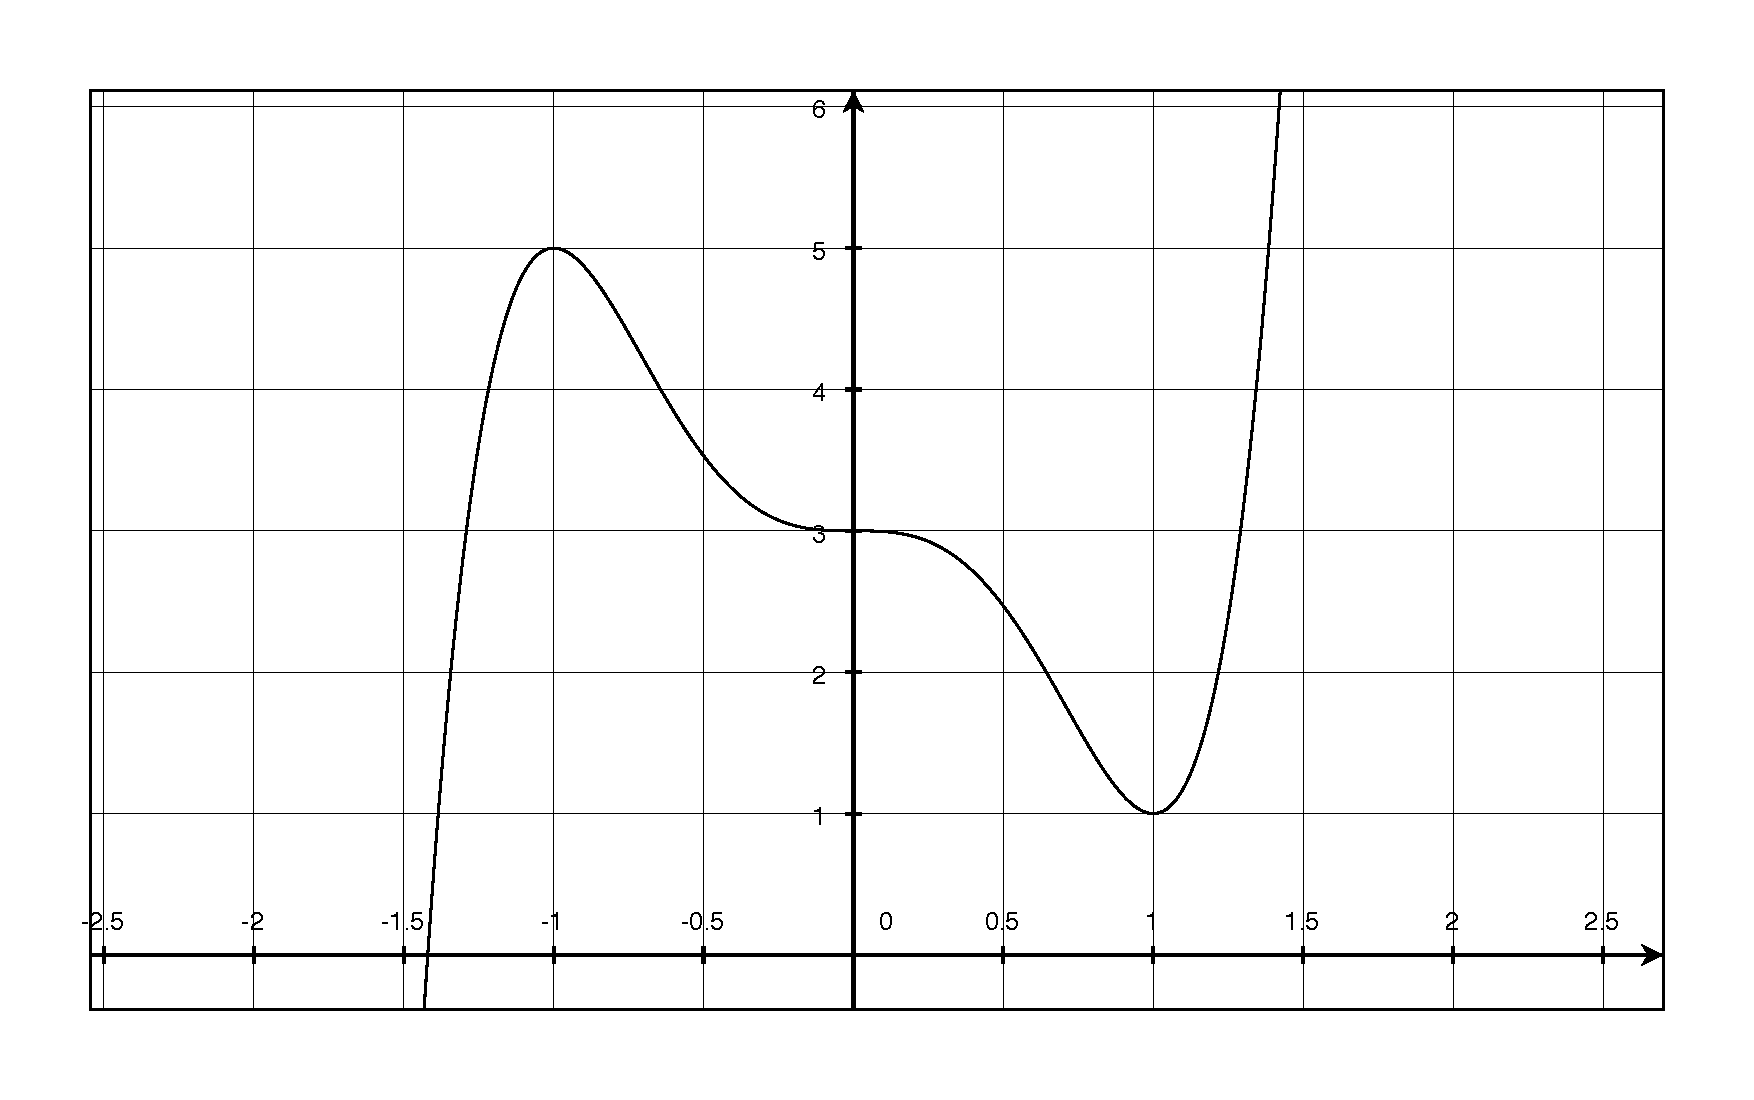
\includegraphics[scale=.3]{final_7_q16.eps}
  \caption*{Question 16}
\end{figure}
\end{solution}

\end{parts}

\ifprintanswers
\pagebreak
\fi

\question
\[
  y = \frac{x}{x - 1}
\]
\begin{parts}
\part Find the vertical and horizontal asymptotes, if any.
\begin{solution}
Since the denominator is zero when $x = 1$, there is a vertical asymptote at $x = 1$

Since $\lim_{x \to \pm\infty} f(x) = 1$, there is a horizontal asymptote at $y = 1$
\end{solution}

\part Find the intervals on which $f$ is increasing or decreasing. 
\begin{solution}
find the derivative:
\begin{align*}
  f'(x) &= \frac{(x - 1) - x}{(x - 1)^2} \\
        &= \frac{-1}{(x - 1)^2} \\
\end{align*}

Since $f'(x)$ is always negative, $f$ is decreasing everywhere except at $x = 1$ where it is not defined.

\end{solution}

\part Find the local maximum and minimum values of $f$.
\begin{solution}
Since $f$ is always decreasing, there aren't any local minimum or maximum values.
\end{solution}

\part Find the intervals of concavity and the inflection points. 
\begin{solution}
Find the second derivative:
\begin{align*}
  f'(x) &= - (x - 1)^{-2}\\
  f''(x) &= 2(x - 1)^{-3} \\
         &= \frac{2}{(x - 1)^3} \\
\end{align*}
The only inflection point occurs when the denominator is zero at $x = 1$.
\begin{itemize*}
  \item concave up: $(1, \infty)$
  \item concave down: $(-\infty, 1)$
\end{itemize*}

\end{solution}

\part Use the information from (a) - (d) to sketch the graph.
\begin{solution}
\begin{figure}[H]
  \centering
  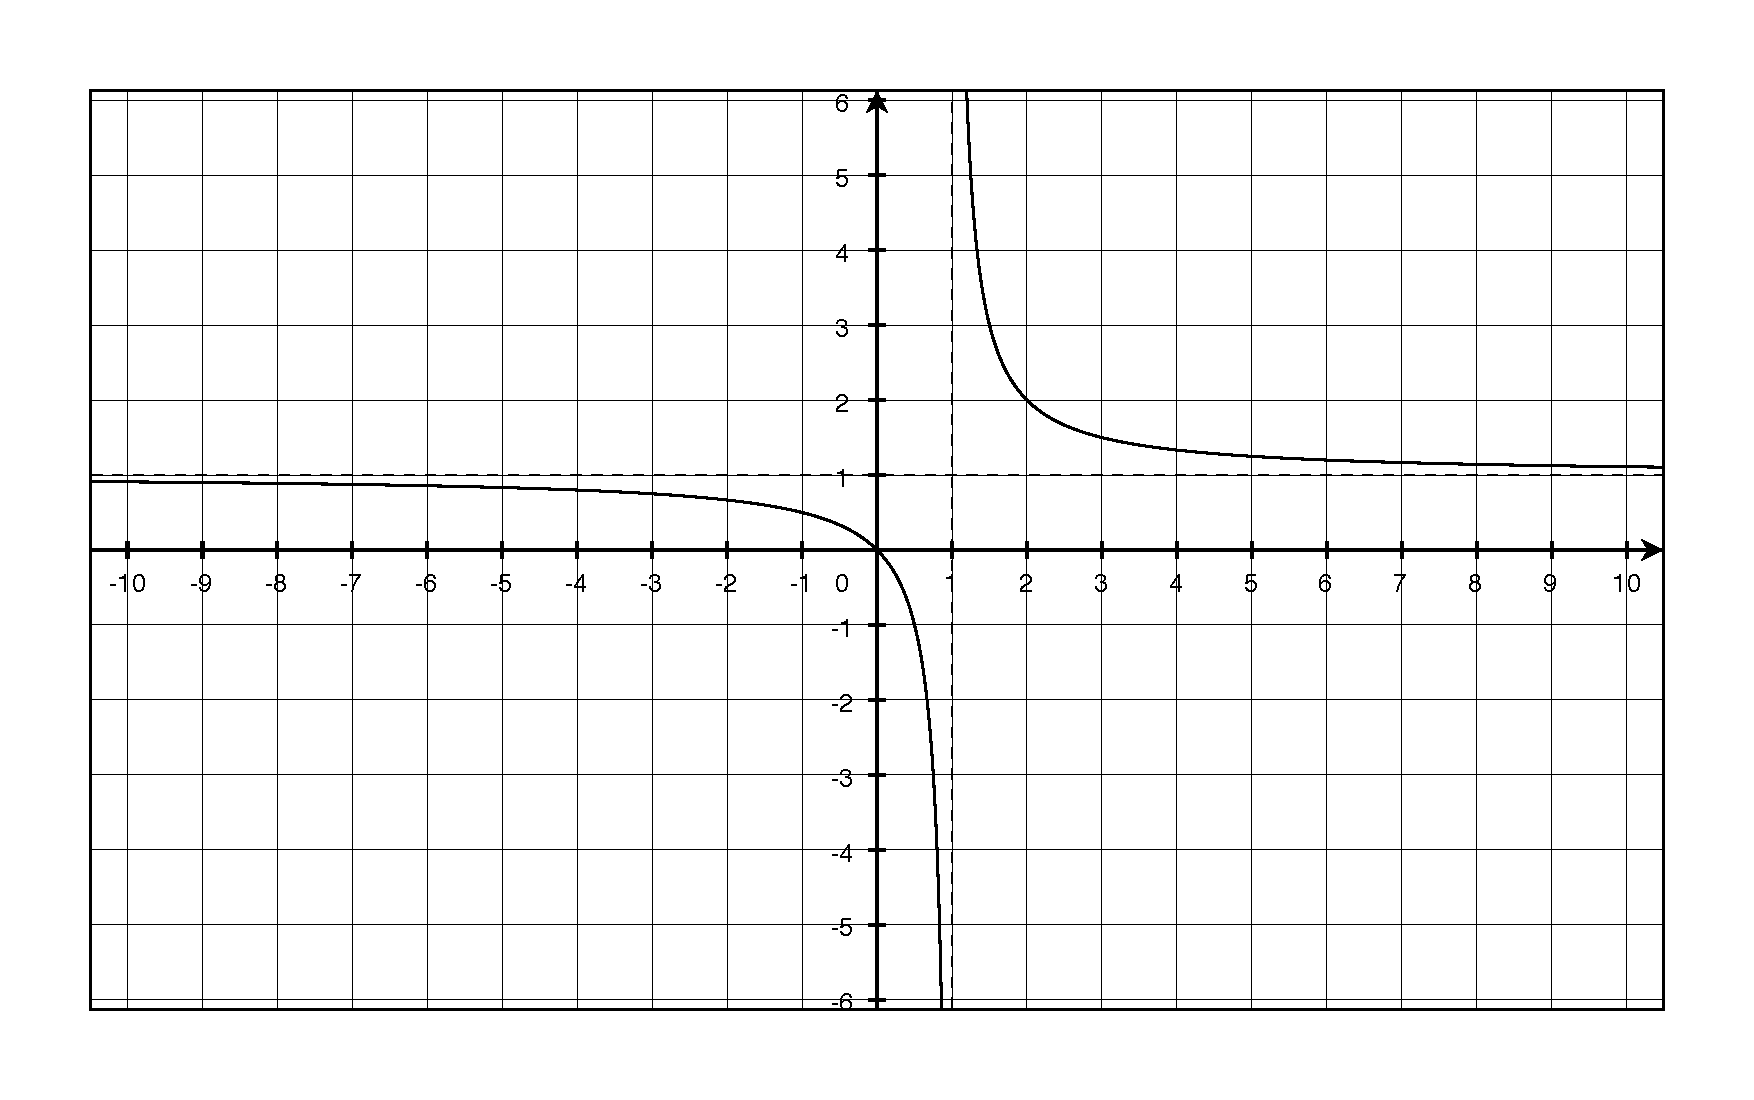
\includegraphics[scale=.3]{final_7_q17.eps}
  \caption*{Question 17}
\end{figure}
\end{solution}

\end{parts}



\end{questions}

\end{document}
